

The last definition we need is the notion of generators (see e.g.~\cite{KelkScornavacca2011}), which we use to describe the underlying structure of networks without nontrivial pendant subtrees. A (binary) \emph{$r$-reticulation generator} is defined as an acyclic directed multigraph with a single root with indegree 0 and outdegree 1, exactly~$r$ nodes with indegree~2 and outdegree at most~1, and all other nodes have indegree 1 and outdegree 2. If~$N$ is a network, then the \emph{underlying generator} of~$N$ is the generator obtained from~$N$ by deleting all leaves and suppressing all indegree 1 outdegree 1 nodes. The \emph{sides} of a generator are its edges (the \emph{edge sides}) and its nodes with indegree 2 and outdegree 0 (the \emph{node sides}). Thus, each leaf of a network~$N$ is on a certain side of its underlying generator. See Figure~\ref{fig:generator} for an example.

\begin{figure}[h]
 \centering
  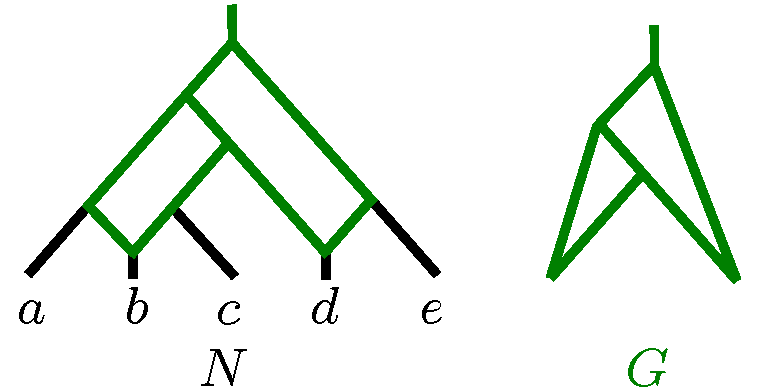
\includegraphics[scale=.5]{../figs/ch4/generator.pdf}
 \caption{Graph $G$ is the generator underlying network $N$. It has 9 sides: 7 edge sides and 2 node sides.}
 \label{fig:generator}
\end{figure}




\section{...drop here unsorted remarks so far}

\begin{enumerate}
 \item To synchronise with the agreement forest literature, and without loss of generality, it will be helpful to sometimes assume that a tree has an artificial vertex, labelled $\rho \not \in X$, which is connected to the original root of the tree (see e.g. Figure~\ref{fig:intro}). We then define $\cL(\cT) = X \cup \{\rho\}$
 \item For an introduction to FPT we refer to \cite{downey1999,Flum2006,Gramm2008,niedermeier2006}.
 \item A \emph{feedback vertex set (FVS)} of a directed graph~$D$ is a subset of the vertices that contains at least one vertex from each directed cycle in~$D$. Equivalently, a subset~$V'$ of the vertices of~$D$ is a feedback vertex set if and only if removing~$V'$ from~$D$ gives a directed acyclic graph. The \emph{minimum feedback vertex set problem on directed graphs} (DFVS) is defined as: given a directed graph~$D$, find a feedback vertex set of~$D$ that has minimum size.
\end{enumerate}



\section{nonbinary intro}

\emph{Background.} A rooted phylogenetic tree is a rooted tree with its leaves labelled by species, or strains of species, more abstractly
known as \emph{taxa}. Arcs, also called edges, are directed away from the root towards the leaves and internal vertices of the tree have indegree~1. It is a model used to exhibit ancestral relations between the species. For an
introduction to phylogenetic trees see \cite{MathEvPhyl,reconstructingevolution,SempleSteel2003}.

Occasionally it happens that on the same set of species topologically distinct phylogenetic trees are derived from different data sources (e.g. different genes). Such partly incompatible trees may arise due to biological reticulation events such as hybridization, recombination or lateral gene transfer \cite{HusonRuppScornavacca10,davidbook,Nakhleh2009ProbSolv}. These events cannot be explained in a tree-like ancestral relation model. There are additionally many non-reticulate biological phenomena, such as incomplete lineage sorting, that can likewise lead to conflicting tree signals  \cite{davidbook,Nakhleh2009ProbSolv}. Whatever the cause of the conflict, it is natural to wish to quantify the dissimilarity of two phylogenetic trees.

\emph{rSPR distance and Maximum Agreement Forests}. One
such measure of dissimilarity is the rooted Subtree Prune and Regraft (rSPR) distance, which asks for the minimum number of subtrees that need to be successively detached and re-attached in one of the trees to transform it into the other. The search for an alternative characterisation of rSPR distance was a major motivation behind the study of the agreement forest problem that
we now describe; a formal definition follows in the next section. We are given two rooted trees with the leaves labeled by the elements of a set~$X$ and no vertices with indegree and outdegree both equal to~1. An \emph{agreement
forest} is a partition of $X$ such that (a) in both trees the partition induces edge-disjoint subtrees and (b) for each block (``component'') of the partition, the two subtrees induced are 
phylogenetically compatible i.e. have a \emph{common
refinement}; see Figure~\ref{fig:maf}. The {\em maximum agreement forest problem} (\maf) is to find an agreement forest with a minimum number of components.




\emph{Hybridization number and Maximum Acyclic Agreement Forests}. The other problem we study is a variation of \maf in which the roots of the subtrees in the agreement forest are not allowed to have conflicting ancestral relations in the two input phylogenetic trees. For an example, consider the agreement forest in Figure~\ref{fig:maf}. In the first phylogenetic tree, the subtree with leaves~$c$ and~$d$ is ``above'' the subtree with leaves~$a$ and~$b$, whereas it is the other way around in the second phylogenetic tree. By saying that a subtree is ``above'' another subtree, we mean that there exists a directed path from the root of the first to the root of the second subtree that contains at least one edge of the first subtree. Hence, the agreement forest in Figure~\ref{fig:maf} is, in this sense, cyclic. Such cyclic phenomena are prohibited in the {\em Maximum Acyclic Agreement Forest problem} \maaf, introduced in \cite{baroni05}. The main reason for studying \maaf, is its close connection with the \emph{
hybridization number problem} (\textsc{hn}). A hybridization network (often also called a rooted phylogenetic network) can informally be thought of as a rooted phylogenetic tree that additionally may contain \emph{reticulations}, vertices with indegree two or higher. Given two rooted trees on the same set of taxa, the \textsc{hn} problem asks for a hybridization network with a minimum number of reticulations that displays (i.e. contains embeddings of) both the input trees. The \textsc{hn} problem can thus be viewed as constructing a ``most parsimonious'' explicit evolutionary hypothesis to explain the dissimilarity between the two input trees; the problem first gained attention following the publication of several seminal articles in 2004-5 e.g. \cite{baroni05,BaroniEtAl2004}. The number of reticulations in an optimal solution to the \textsc{hn} problem is exactly one less than the number of components in an optimal solution to the \maaf problem \cite{baroni05}, making the problems essentially equivalent.

{Preliminaries and statement of results}\label{sec:prelim}
Let~$X$ be a finite set (e.g. of species). A \emph{rooted phylogenetic} $\cX$-\emph{tree} is a rooted tree \textcolor{red}{with at least three vertices}, no vertices with indegree-1 and outdegree-1, a root with indegree-0 and outdegree at least~2, and leaves bijectively labeled by the elements of~$X$. We identify each leaf with its label. We henceforth call a rooted phylogenetic $X$-tree a \emph{tree} for short. Note that we do not restrict phylogenetic trees to be binary. A tree~$T$ is a \emph{refinement} of a tree~$T'$ if~$T'$ can be obtained from~$T$ by contracting edges. For a tree~$T$ and a set $X'\subset X$, we define $T(X')$ as the minimal subtree of~$T$ that contains all elements of~$X'$, and $T|X'$ as the result of suppressing all vertices with in- and outdegree~1 of~$T(X')$. The set of leaves of a tree~$T$ is denoted~$L(T)$. We say that tree~$T'$ is displayed by tree~$T$ if~$T'$ can be obtained from a subtree of~$T$ by contracting edges. If~$T'$ is displayed by~$T$, then $T(L(T'))$ is the \emph{
embedding} of~$T'$ in~$T$.

Throughout the thesis, we usually refer to directed edges (arcs) simply as edges and to directed paths simply as paths. If~$e=(u,v)$ is an edge of some tree, then we say that~$v$ is a \emph{child} of~$u$, that~$u$ is the \emph{parent} of~$v$, that~$u$ is the \emph{tail} of~$e$, that~$v$ is the \emph{head} of~$e$ and we write $tail(e)=u$ and $head(e)=v$.



\section{Background: BMC practical cyclekiller}

{Phylogenetic trees are} used in biology to represent the evolutionary history of a set ${\cX}$ of species (or \emph{taxa}) \cite{MathEvPhyl,reconstructingevolution}. They are trees whose leaves are bijectively labeled by ${\cX}$ and whose internal vertices represent the ancestors of the species set; they can be rooted or unrooted. Since in a rooted tree edges have a direction, the concepts of indegree and outdegree of a vertex are well defined. \emph{Binary} rooted (phylogenetic)  trees are rooted (phylogenetic) trees whose internal vertices have outdegree~2. \emph{Nonbinary} rooted (phylogenetic) trees have no restriction on the outdegree of inner vertices.

Biological events in which a species derives its genes from different ancestors, such as hybridization, recombination and horizontal gene transfer events, cannot be modelled by a tree. To be able to represent such events, a generalization of trees is considered which allows vertices with indegree two or higher, known as \emph{reticulations}. This model, which is called a \emph{{rooted} phylogenetic network}, is of growing importance to biologists~\cite{bapteste}. For detailed background information we refer the reader to \cite{HusonRuppScornavacca10,surveycombinatorial2011,Nakhleh2009ProbSolv}.

{Although phylogenetic networks are more general than phylogenetic trees, trees are still often the basic building blocks from which phylogenetic networks are constructed. Specifically, there are many techniques available for constructing gene trees. However, when more genes are analyzed, topological conflicts between individual gene phylogenies can arise for methodological or biological reasons (e.g. aforementioned reticulate phenomena such as hybridization). This has led computational biologists to try and quantify the amount of reticulation that is needed to simultaneously explain two trees.

To state this problem more formally, {we have that a  phylogenetic tree~$T$ on~$\cX$ is a refinement of a  phylogenetic tree~$T'$ on the same set~$\cX$ if $T$ can be obtained from $T'$ by deleting edges and identifying their incident vertices. Then,} 
we say that a phylogenetic network~$N$ on~$\cX$ \emph{displays} a phylogenetic tree~$T$ on~$\cX$ if~$T$ can be obtained from a subgraph of~$N$ by contracting edges. Informally, this means that (a refinement of)~$T$ can be obtained from~$N$ by, for each reticulation vertex of~$N$, ``switching off'' all but one of its incoming edges and then suppressing all indegree-1 outdegree-1 vertices ({i.e. replacing paths of these vertices by one edge}). Given two rooted phylogenetic trees~$T_1$ and~$T_2$ on~$\cX$, the problem then becomes to determine the minimum number of reticulation events contained in a phylogenetic network~$N$ on~$\cX$ displaying both trees (where an indegree-$d$ reticulation counts as~$d-1$ reticulation events). The value we are minimizing is often called the \emph{hybridization number} and instead of the term phylogenetic network, the term \emph{hybridization network} is often used. It is known that the problem of computing hybridization numbers is both NP-hard and APX-hard~\cite{
bordewich07a}, but it is not known whether it is in APX (i.e. whether it admits a polynomial-time approximation algorithm that achieves a constant approximation ratio).

Until recently, most research on the hybridization number of two phylogenetic trees had focused on the question of how to exactly compute this value using fixed parameter tractable (FPT) algorithms, where the parameter in question is the hybridization number~$r$ of the two trees. For an introduction to FPT we refer to~\cite{Flum2006,DowneyFellows99}.

For binary trees, algorithmic progress has been considerable in this area, with various authors reporting increasingly sophisticated FPT algorithms~\cite{bordewich2,hybridnet,quantifyingreticulation,whiddenFixed}. The fastest algorithms currently implemented are the algorithm available inside the package \textsc{Dendroscope}~\cite{Dendroscope3}, based on~\cite{fastcomputation}, and the sequence of progressively faster algorithms in the \textsc{HybridNet} family~\cite{hybridnet,chen2012algorithms,chen2013ultrafast}. The fastest theoretical FPT algorithm has running time $O( 3.18^{r}n )$ \cite{whiddenFixed}, where~$n$ is the number of taxa in the trees.

Even though in practice it rarely happens that trees are binary, the nonbinary variant of the problem has been less studied. The nonbinary version is also FPT \cite{linzsemple2009,terminusest} and a (non-FPT) algorithm has recently been implemented in \textsc{Dendroscope}~\cite{Dendroscope3}.

Such (FPT) algorithms do, however, have their limits. The running time still grows exponentially in~$r$, albeit usually at a slower rate than algorithms that have a running time of the form $n^{f(r)}$, where~$f$ is some function of~$r$. In practice this means that existing algorithms can only handle instances of binary trees when~$r$ is at most 40-50 and instances of nonbinary trees when~$r$ is at most 5-10.

These limitations are problematic. Due to ongoing advances in DNA sequencing, more and more species and strains are being sequenced. Consequently, biologists use trees with more and more taxa and software that can handle large trees is required. For such large and/or difficult trees one can try to generate heuristic or approximate solutions, but how far are such solutions from optimality? In~\cite{cyclekiller} we showed that the news is worrying. Indeed, we showed that polynomial-time constant-ratio approximation algorithms exist if and only if such algorithms exist for the problem Directed Feedback Vertex Set (DFVS). However, DFVS is a well-studied problem in combinatorial optimization and to this day it is unknown if it permits such an algorithm. Pending a major breakthrough in computer science, it therefore seems difficult to build polynomial-time algorithms which approximate hybridization number well. On the positive side, we showed that in polynomial time an algorithm with approximation ratio $O(\log r \
log \log r)$ is possible. However, this algorithm is purely of theoretical interest and is not useful in practice.






\subsection{survay like things...}
The binary \maf problem, in which the two input phylogenetic trees are binary, was introduced by Hein et al.~\cite{hein96}. Bordewich and Semple~\cite{BS05} showed that modulo a minor rooting technicality it is equivalent to computing the rSPR distance. The first correct polynomial-time approximation algorithm for this problem was the 5-approximation algorithm by Bonet et al.~\cite{bonet}. The first 3-approximation was given in~\cite{rsprFPT}, a quadratic-time 3-approximation in~\cite{3approxRSPR} and a linear-time 3-approximation in~\cite{whiddenFixed}. A fixed parameter tractable (FPT) algorithm for binary \maf was first given by Bordewich and Semple~\cite{BS05}, the running time of which was subsequently improved in~\cite{rsprFPT} to $O(4^kk^4+n^3)$ and in~\cite{whiddenFixed} to $O(2.42^kn)$. (See \cite{Flum2006,niedermeier2006} for an introduction to fixed parameter tractability). For more than two binary trees, there exists an 8-approximation~\cite{chataigner}.


The close relationship between rSPR distance and \maf also holds in the nonbinary case~\cite{josh}. However, compared to the binary case neither problem has been well-studied. Nonbinary agreement forests were introduced in~\cite{3approxRSPR}, where a $(d+1)$-approximation algorithm for nonbinary \maf was given, with~$d$ the maximum outdegree of the input trees. A kernelization was presented in~\cite{josh}, showing that nonbinary \maf is fixed-parameter tractable. Combining this kernelization of size~$64k$ with the trivial $O(n^k\text{poly}(n))$ time exact algorithm gives a $O((64k)^k\poly(n))$ time FPT algorithm, with~$n$ the number of species and~$k$ the size of the maximum agreement forest minus one. In addition, the kernel automatically implies the existence of a polynomial-time 64-approximation algorithm (since any instance trivially has a solution of size~$n$).


In this article we give a polynomial-time 4-approximation algorithm and an $O(4^k \poly(n))$ time FPT algorithm for nonbinary \maf. Both algorithms have been implemented and made publicly available. Although these results are of interest in their own right, we also show how to utilize them to obtain improved algorithms for computation of hybridization number.